\documentclass[a4paper]{article}

\usepackage{fullpage} % Package to use full page
\usepackage{parskip} % Package to tweak paragraph skipping
\usepackage{amsmath}
\usepackage{hyperref}
\usepackage{amsmath,amsfonts,amsthm} % Math packages
\usepackage{graphicx}
\usepackage{listings}
\usepackage{color}
\usepackage{float}
\definecolor{codegreen}{rgb}{0,0.6,0}
\definecolor{codegray}{rgb}{0.5,0.5,0.5}
\definecolor{codepurple}{rgb}{0.58,0,0.82}
\definecolor{backcolour}{rgb}{0.95,0.95,0.92}
\definecolor{brown}{rgb}{0.59, 0.29, 0.0}
\definecolor{beaublue}{rgb}{0.74, 0.83, 0.9}
\definecolor{orange}{rgb}{1.0, 0.5, 0.0}
\definecolor{darkslategray}{rgb}{0.18, 0.31, 0.31}
\def\Xint#1{\mathchoice
	{\XXint\displaystyle\textstyle{#1}}%
	{\XXint\textstyle\scriptstyle{#1}}%
	{\XXint\scriptstyle\scriptscriptstyle{#1}}%
	{\XXint\scriptscriptstyle\scriptscriptstyle{#1}}%
	\!\int}
\def\XXint#1#2#3{{\setbox0=\hbox{$#1{#2#3}{\int}$}
		\vcenter{\hbox{$#2#3$}}\kern-.5\wd0}}
\def\dashint{\Xint-}

% Swap the definition of \abs* and \norm*, so that \abs
% and \norm resizes the size of the brackets, and the 
% starred version does not.
\makeatletter
\let\oldabs\abs
\def\abs{\@ifstar{\oldabs}{\oldabs*}}
%
\let\oldnorm\norm
\def\norm{\@ifstar{\oldnorm}{\oldnorm*}}
\makeatother
\lstdefinestyle{mystyle}{
	backgroundcolor=\color{white},   
	commentstyle=\color{codegreen},
	keywordstyle=\color{blue},
	identifierstyle=\color{brown},
	numberstyle=\tiny\color{codegray},
	stringstyle=\color{orange},
	basicstyle=\footnotesize,
	breakatwhitespace=false,         
	breaklines=true,                 
	captionpos=b,                    
	keepspaces=true,                 
	numbers=left,                    
	numbersep=5pt,                  
	showspaces=false,                
	showstringspaces=false,
	showtabs=false,                  
	tabsize=2
}
\lstset{style=mystyle}

\title{AMATH 575: Problem Set 1}
\author{Jithin D. George, No. 1622555}
%\date{23/11/16}
% matrix environment
\newenvironment{mat}{\left[ \begin{array}{ccccccccccccc}}{\end{array}\right]}
\newcommand\bcm{\begin{mat}}
	\newcommand\ecm{\end{mat}}

\begin{document}

\maketitle
\begin{enumerate}

	
	\item 
	
\[\dot{x} = y \]
\[ \dot{y} = - \delta y - \mu x - x^3 \]
$\mu$ is 1.
The fixed points are (0,0), (i,0) and (-i,0)

The jacobian is given by 
\[ \bcm   0 & 1\\ -1 -3x^2 &-\delta  \ecm \]

For (0,0), this is 
\[ \bcm   0 & 1\\ -1 &-\delta  \ecm \]

\[\lambda_1 = \frac{1}{2}(-\sqrt{\delta^2-4} -\delta) \]
\[\lambda_2 = \frac{1}{2}(\sqrt{\delta^2-4} -\delta) \]

For the real part of both these eigenvalues to be negative, $\delta$ has to be positive.

So, for positive $\delta$, (0,0)is stable.
For negative $\delta$, (0,0)is unstable.
For $ \delta$ = 0, the eigenvalues are complex and we can't say anything about their stability.

For (i,0) and (-i,0), this is 
\[ \bcm   0 & 1\\ 2 &-\delta  \ecm \]

\[\lambda_1 = \frac{1}{2}(-\sqrt{\delta^2+8} -\delta) \]
\[\lambda_2 = \frac{1}{2}(\sqrt{\delta^2+8} -\delta) \]

As long as $\delta$ is real, $ \lambda_2$ will always have a positive real part. So, (i,0) and (-i,0) are always unstable fixed points.


\item 

\[\dot{r}= r(1-r^2)\]
\[\dot{\theta}= cos(4\theta)\]
The fixed points given the constraints on r and $\theta$ are (0,$\frac{\pi}{8}$),(0,$\frac{3\pi}{8}$), (0,$\frac{5 \pi}{8}$), (0,$\frac{7\pi}{8}$), (0,$\frac{9\pi}{8}$),(0,$\frac{11\pi}{8}$), (0,$\frac{13\pi}{8}$), (0,$\frac{15\pi}{8}$),(1,$\frac{\pi}{8}$),(1,$\frac{3\pi}{8}$), (1,$\frac{5 \pi}{8}$), (1,$\frac{7\pi}{8}$), (1,$\frac{9\pi}{8}$),(1,$\frac{11\pi}{8}$), (1,$\frac{13\pi}{8}$) and (1,$\frac{15\pi}{8}$).
The Jacobian is 
\[\bcm 1-3r^2 & 0\\0  &- 4sin(4\theta)  \ecm \]

When r= 0, the maximal eigenvalue is 1 and it is clearly unstable. When r= 1,
it depends on the sign of $sin(4\theta)$

\vspace{90mm}
\item 
\[ x' = 10(-x+y) \]
\[ y' = rx -y -xz \]
\[ z' = -\frac{8}{3}z +xy\]
The fixed points are (0,0,0)($\sqrt{\frac{8}{3}(r-1)},\sqrt{\frac{8}{3}(r-1)},r-1$ )
and ($-\sqrt{\frac{8}{3}(r-1)},-\sqrt{\frac{8}{3}(r-1)},r-1$ )

The jacobian is given by 
\[\bcm -10 & 10 & 0\\r-z &-1 &-x \\ y &x &-8/3 \ecm \]

For the first fixed point, this becomes
\[\bcm -10 & 10 & 0\\r &-1 & 0 \\ 0 &0  &-8/3 \ecm \]
We can see the eigenvalues $-\frac{8}{3}$, $\frac{1}{2}(\sqrt{40r+81}-11)$ and  $\frac{1}{2}(-\sqrt{40r+81}-11)$. So, (0,0,0)is an asymptotically stable fixed point if r $<$1 , unstable if r$>$1 and of unknown stability if r =1.


For the second  fixed point, the jacobian becomes
\[\bcm -10 & 10 & 0\\1 &-1 &-\sqrt{\frac{8}{3}(r-1)} \\ \sqrt{\frac{8}{3}(r-1)} &\sqrt{\frac{8}{3}(r-1)} &-8/3 \ecm \]

\[\lambda^3 + \frac{41 \lambda^2}{3} + \frac{80 \lambda}{3} + \frac{8 \lambda r}{3} + \frac{160 (r-1)}{3}  =0\]

We get the same characteristic equation for the third fixed point as well.

For ($\sqrt{\frac{8}{3}(r-1)},\sqrt{\frac{8}{3}(r-1)},r-1$ )
and ($-\sqrt{\frac{8}{3}(r-1)},-\sqrt{\frac{8}{3}(r-1)},r-1$ ) to be stable, by the Routh-Hurwtiz table, we need
\[\frac{160(r-1)}{3}>0, 41(80+80r)-480(r-1)>0   \]

Thus, for those points to be stable, r has to between 1 and $\frac{470}{19}$. 


\item
\[\theta_{n+1} = \theta_{n} + I_n - \frac{K}{2\pi}sin2\pi\theta_{n} mod 1\]
\[I_{n+1} =  I_n - \frac{K}{2\pi}sin2\pi\theta_{n} \]
 The expression we get after taking th determinant to find the eigenvalues is 
The mod makes theta periodic between 0 and 1.
The jacobian is given by
\[ \bcm 1 - Kcos 2\pi \theta & 1  \\ - Kcos 2\pi \theta & 1 \ecm \]
If K=0, the fixed points are at ($\theta$,n) where n is any integer and $\theta$ lies in [0,1).
The jacobian becomes 
\[ \bcm 1  & 1  \\ 0 & 1 \ecm \]
The eigenvalues are 1. So, we need higher order terms for stability. 
Otherwise, the fixed points are at (0,0) and (0,$\frac{1}{2}$). The fixed point at (0,1) does not exist because of the mod.
\[ \bcm 1 - K & 1  \\ - K & 1 \ecm \]
The eigenvalues are given by
\[ \lambda = \frac{1}{2}(2 - k \pm \sqrt{k^2-4k}) \]
We plot the bigger eigenvalue.
\begin{figure}[h!] 
	\centering
	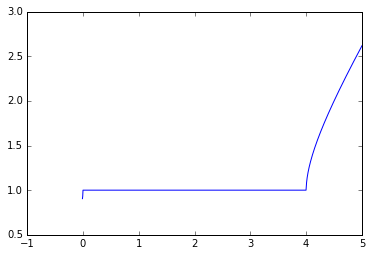
\includegraphics[width=8cm]{map1}
\end{figure}


We can see that, for K $>$ 4, the absolute value of the maximal eigenvalue is greater than 1 and both the fixed points are unstable (saddle).
For K in between 0 and 4, the eigenvalues are 1 and we would need the higher order terms to find the stability.
\item
\textbf{Flow}:
\[\dot{x} = x^2 +y^2\]
\[\dot{y} = x^2 +y^2\]

At the fixed point (0,0), the jacobian is 
\[\bcm 0 &0 \\ 0& 0 \ecm\]
The eigenvalues are (0,0) indicating a center. However, for any value of x and y, $\dot{x}$ and $\dot{y}$ $>$0. So, it is clearly non-linearly unstable.

\textbf{Map}:
\[x_{n+1} =x_n+ x_n^2 +y_n^2\]
\[y_{n+1} =y_n+ x_n^2 +y_n^2\]

At the fixed point (0,0), the jacobian is 
\[\bcm 1 &0 \\ 0& 1 \ecm\]
The eigenvalues are (1,1) indicating a center. However, for any value of x and y, $x_{n+1} >x_n$ and $y_{n+1} >y_n$. So, it is clearly non-linearly unstable.
\item 
\[\dot{\theta}= 1 + sin^2 \theta + (1-r)^2 \]
\[ \dot{r} = r(1-r)\]

\begin{figure}[h!] 
	\centering
	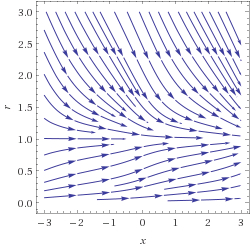
\includegraphics[width=4cm]{q_6}
\end{figure}

If we define the distance between two points ($r_1,\theta_1$)and ($r_2,\theta_2$)
\[a^2 = (r_1- r_2)^2+ (\theta_1- \theta_2)^2\]
We get 
\[\frac{da^2}{dt} = (r_1- r_2)^2+ (\theta_1- \theta_2)^2\]
\[= 2(r_1- r_2)(r'_1- r'_2)+ 2(\theta_1- \theta_2)(\theta'_1- \theta'_2)\]
\[ = 2(r_1- r_2)(r_1-r_1^2- r_2+ r_2^2)+ 2(\theta_1- \theta_2)(sin^2(\theta_1)- sin^2(\theta_2) +r_1^2-r_2^2-2r_1+2r_2)\]
\[ = 2(r_1- r_2)^2(1-r_1- r_2)+ 2(\theta_1- \theta_2)((sin(\theta_1)- sin(\theta_2))(sin(\theta_1)+ sin(\theta_2)) + (r_1- r_2)(1-r_1- r_2))\]
Using $|sin(\theta_1)-sin(\theta_2)|\leq |(\theta_1)-(\theta_2)|$
\[ \leq 2(r_1- r_2)^2(1-r_1- r_2)+ 2(\theta_1- \theta_2)((\theta_1- \theta_2)(sin(\theta_1)+ sin(\theta_2)) + (r_1- r_2)(1-r_1- r_2))\]
Using $|(\theta_1)-(\theta_2)|\leq a$ and $|(r_1)-(r_2)|\leq a$
\[ \leq 2a^2(1-r_1- r_2)+ 2a(a(sin(\theta_1)+ sin(\theta_2)) + a(1-r_1- r_2))\]
\[ \leq  2a^2(sin(\theta_1)+ sin(\theta_2) + 2(1-(r_1+ r_2)))\]
Since $|r_1|\leq max(1,r_0)$ because trajectories seem to go to r=1,
\[ \leq  2a^2(4-(r_{01}+ r_{02}))\]
\[ \frac{da^2}{dt}\leq  Ka^2\]
Since the distance is bounded in this fashion, we have a bound on the distance. So given two points initially separated by a $\delta$, we can find a bound on the $\epsilon$, the distance between them for the rest of time. Thus, this system is orbitally stable.
\item
The general solution is spanned by 
	\[\bcm x \\ y\\ z\ecm = -11  \bcm -10 \\1 \\0 \ecm - \frac{8}{3}  \bcm 0\\0 \\1\ecm+ 0 \bcm 1\\1 \\0 \ecm \]
The dimension of the stable manifold is 2 while that of the center manifold is 1. 
The stable manifold is in the form
\[ y= a x + bz + c x^2 + d z^2 + e xz + O(x^3)\]

\[y'= (a+2cx+ez)x'  + (b+2dz+ex)z' \]
\[x-y-xz= (a+2cx+ez)(-10x+10y)  + (b+2dz+ex)(-\frac{8}{3}z+xy) \]

\[-30 a^2 x - 3 a b x^2 - 30 a b z - 90 a c x^2 - 6 a d x^2 z - 30 a d z^2 - 3 a e x^3 - 60 a e x z + 27 a x - 3 b^2 x z - 3 b c x^3 - 60 b c x z \]
\[ - 9 b d x z^2 - 6 b e x^2 z - 30 b e z^2 + 5 b z - 60 c^2 x^3 - 6 c d x^3 z - 60 c d x z^2 - 3 c e x^4 - 90 c e x^2 z + 57 c x^2\]\[ - 6 d^2 x z^3 - 9 d e x^2 z^2 - 30 d e z^3 + 13 d z^2 - 3 e^2 x^3 z - 30 e^2 x z^2 + 35 e x z - 3 x z + 3 x=0\]
Equating coefficients, we have
\[a= 1,-\frac{1}{10} \]
\[b=0, c =0, d=0 \]
\[e = \frac{3}{41}, -\frac{3}{25}\]
The stable manifold is given by the appropriate coefficients
\[ y = -\frac{1}{10}x -\frac{3}{25} xz \]

For the center manifold, we express

\[y = h_1(x) = a x + b x^2\]
\[z = h_2(x) = cx +dx^2 \]

\[y' = (a+2bx)x'\]
\[z' = (c+2dx)x'\]

\[x-y-xz = (a+2bx)(-10x+10y) \]
\[x-(a x + b x^2)-x( cx +dx^2) = (a+2bx)(-10x+10(a x + b x^2)) \]
\[-\frac{8}{3}z+xy = (c+2dx)(-10x+10y)\]
\[-\frac{8}{3}(cx +dx^2)+x(a x + b x^2) = (c+2dx)(-10x+10(a x + b x^2))\]
Equating coefficients, we have
\[a= 1,-\frac{1}{10} \]
\[b=0, c =0,  \]
\[d = \frac{3}{500}, \frac{3}{8}\]
The center manifold is given by the appropriate coefficients
\[ y = x \]
\[ z = \frac{3}{8} x^2 =\frac{3}{8} y^2  \]

The unstable manifold is the empty set.
\item 
At the saddle points, the dimension of the stable manifold is 1 and that of the unstable manifold is 1 (and center 0).
The manifold would be of the form 
\[\theta_{n+1} = aI_{n+1} + bI^2_{n+1} + \ldots \]
\[\theta_{n}+I_n - K\theta_n = a(I_n - K\theta_n) + b(I_n - K\theta_n)^2 + \ldots \]
\[(a-Ka+1)I_{n} + b(1-K)I^2_{n}  = a(I_n - K(aI_{n} + bI^2_{n})) + b(I_n - K(aI_{n} + bI^2_{n}))^2 + \ldots \]

\[a= \frac{\sqrt{K} - \sqrt{K - 4}}{2 \sqrt{K}}, \frac{\sqrt{K} + \sqrt{K - 4}}{2 \sqrt{K}}\]
\[b=0\]

Thus, the stable manifold would be
\[\theta_{n} = \frac{\sqrt{K} - \sqrt{K - 4}}{2 \sqrt{K}}I_{n}\]

The unstable manifold would be
\[\theta_{n} = \frac{\sqrt{K} + \sqrt{K - 4}}{2 \sqrt{K}}I_{n}\]

\item 

\begin{enumerate}
	\item
	\[\frac{dy}{dx} =\frac{dy}{dt}\frac{dt}{dx} = \frac{-2x^2+2xy^2}{-x+y^2}  = 2x\]
	\[y = x^2 +c \]

	Thus, $y =x^2$ is an invariant manifold because it is a solution curve to the systems of 2 odes.
	\item
	\[\dot{x}= -x +y^2\]
	Plugging in y = $x^2$,
	\[\dot{x}= -x +x^4\]
	The solution to this is 
	\[x(t) = {\frac{1}{(e^{c_1 + 3 t} + 1)}}^{1/3}\]
	As t goes from $-\infty$ to $\infty$, (x,y) goes from (0,0) to (1,1). Thus , y = $x^2$ is the trajectory connecting (0,0) and (1,1)
	
	\item 
	At (0,0), we get that the eigenvectors give us the following span.
	\[\bcm x \\ y\ecm = -1 \bcm 1 \\0 \ecm + 0 \bcm 0 \\1 \ecm \]
	Thus, we see that the center manifold should be tangent to the y-axis. 
	However, $y = x^2$ is tangent to the x-axis which means it is the stable manifold.
	
\end{enumerate}
	\end{enumerate} 
\end{document}